%!TEX root = ../CombinatoricsNotes.tex

\section{Intersecting hypergraphs}

A family $\F\subset \P([n])$ is \defn{intersecting}[intersecting set system] if every two sets $A,B\in \F$ have $A\cap B\neq \emptyset$. If $\F$ is intersecting, then $|\F| \leq 2^{n-1}$ because $\F$ can contain at most one set in each pair $\{A,A^c\}$ for every $A\subset [n]$. On the other hand, $2^{n-1}$ may be acheived by taking $\F = \{A\subset [n]: x\in A\}$ for some $x\in [n]$.
What if $\F\subset [n]^{(r)}$ for some $r$? If $r> n/2$, then $\F = [n]^{(r)}$ is intersecting.

\begin{theorem}[\cite{erdos-ko-rado-1961}] \label{thm:erdos-ko-rado} 
Let $r \leq n/2$ and $\F\subset[n]^{(r)}$ be intersecting. Then
\[
|\F| \leq {n-1\choose r-1}
\]
which can be acheived by $\F = \{A\in [n]^{(r)}: x\in A\}$ for some $x\in [n]$.
\end{theorem}
\begin{proof}	
Let us consider a particular circular ordering of $[n]$ and upper bound the number of sets in $\F$ which are intervals of size $r$ in this order. 
\begin{figure}[ht]
\usetikzlibrary{fit}
\begin{center}
\begin{tikzpicture}
 \begin{scope}
\node[left] at (0,0) {$\circlearrowleft$};

\foreach \x in {1,...,8}
{
 \pgfmathsetmacro\myangle{\x*45}
\filldraw[black] (\myangle:1cm) circle (0.4pt) node[left]{\x};
}
 \end{scope}
 \node[xshift=45pt] at (0,0) {$=$};
% \end{tikzpicture}
% $=$
% \begin{tikzpicture}
\begin{scope}[xshift=100pt]
\node[left] at (0,0) {$\circlearrowleft$};
\foreach \x in {1,...,8}
{
 \pgfmathsetmacro\myangle{\x*45+45}
\filldraw[black] (\myangle:1cm) circle (0.4pt) node[left]{\x};
}
\end{scope}
 \node[xshift=145pt] at (0,0) {$\neq$};

% \end{tikzpicture}
% $\neq$
% \begin{tikzpicture}
\begin{scope}[xshift=200pt]
\node[left] at (0,0) {$\circlearrowleft$};
\foreach \x in {1,...,8}
{
 \pgfmathsetmacro\myangle{-1*\x*45+90}
\filldraw[black] (\myangle:1cm) circle (0.4pt) node[left]{\x};
}
\end{scope}
\end{tikzpicture}
\end{center}
\caption{An illustration of circular orders on $[8]$. We define our order counter-clockwise, and so the order is invariant under rotations, as the equality between the left and center orders demonstrates. However, the right order was obtained by reversing the order of the left, and thus is a new order.}\label{fig:circ_order}
\end{figure}
Let us prove there are at most $r$ intervals.
Let us fix an interval $I= (a_1,a_2,\dotsc,a_r)$, and count the number of intervals which intersect it. For each pair of consecutive points $(a_{i-1},a_i)$\sidenote{Corresponding to gaps between points} in this interval $I$, there is an interval $I_1$ with first element $a_{i+1}$ and an interval $I_2$ with last element $a_i$, yielding $2(r-1)$ intervals intersecting it. But $\F$ can contain at most one interval in this pair $(I_1,I_2)$, because $I_1\cap I_2=\emptyset$. So we are left with $r-1$ intervals intersecting $I$, along with $I$ itself. Thus, we've found $r$ intersecting intervals in this circular order.

How many circular orders are there on $[n]$? Every circular order corresponds to $n$ permutations (all rotations of each other), and there are $n!$ total permutations, yielding $(n-1)!$ circular orders.

\begin{marginfigure}
\begin{center}
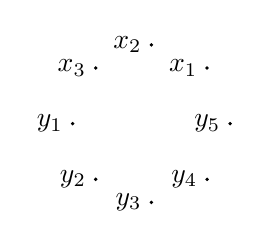
\begin{tikzpicture}
\begin{scope}
\node[left] at (0,0) {$\circlearrowleft$};

\foreach \x in {1,...,3}
{
 \pgfmathsetmacro\myangle{\x*45}
\filldraw[black] (\myangle:1cm) circle (0.4pt) node[left]{$x_{\x}$};
}
\foreach \x in {1,...,5}
{
 \pgfmathsetmacro\myangle{(\x+3)*45}
  % \pgfmathsetmacro\y{\x-3}
\filldraw[black] (\myangle:1cm) circle (0.4pt) node[left]{$y_{\x}$};
}
 \end{scope}
\end{tikzpicture}
\end{center}
\caption{An order in which $X = \{x_1,x_2,x_3\} \in [8]^{(3)}$ is an interval, where we've enumerated $[8]\setminus X = \{y_1,\dotsc,y_5\}$.} \label{fig:X_interval_circ_order}
\end{marginfigure}
In how many circular orders is a given $X\in [n]^{(r)}$ an interval? To obtain an interval, we order the elements of $X$ in $r!$ ways, and then order the rest of the set in $(n-r)!$ ways, yielding $r!(n-r)!$ orders in which $X$ is an interval. See \cref{fig:X_interval_circ_order} for an illustration. 

We have at most $r$ sets of $\F$ as intervals per circular order, and $(n-1)!$ circular orders, so at most $r(n-1)!$ sets in $\F$ over all circular orders.

On the other hand, each set of $\F$ has only $r!(n-r)!$ orders in which it is an interval. Thus, we have $|\F| r!(n-r)!$ intervals corresponding to sets in $\F$, counted over all orders. Hence,
\[
|\F| r! (n-r)! \leq r(n-1)! 
\]
which completes the proof.
\end{proof}

\begin{remark}
For $r < n/2$, if $\F\subset [n]^{(r)}$ is intersecting and has maximal size, i.e. $|\F| = {n-1\choose r-1}$, then for some $x\in n$, we have
\[
\F = \{A\in [n]^{(r)}: x\in A \}.
\]
The proof is left as an exercise. In particular, there are only $n$ possible extremal families.

Consider $r=n/2$. For each set $A \in [n]^{(r)}$, there is only one forbidden set $A^c$. So $\F$ may be formed by choosing one set $A$ from each pair $\{A,A^c\}$ arbitrarily. This yields a doubly-exponential number of extremal families.
\end{remark}

\newthought{We will now consider} a generalization of intersecting.
% \begin{definition}
We say $\F\subset [n]^{(r)}$ is \defn{$t$-intersecting}[t-intersecting] if $|A\cap B|\geq t$ for all $A,B\in \F$.
% \end{definition}
We wish to find $m(n,r,t)$, the maximum size of a $t$-intersecting family $\F$ which is a subset of $[n]^{(r)}$.
A natural guess of an optimal family would be 
\[
 \F_0 := \F_0(n,r,t) = \{ A \in [n]^{(r)}: L\subset A\}
\] for some $L\subset [n]$ with $|L| = t$.
Note $|\F_0| = {n-t \choose r-t}$.
On the other hand, for which $n,r,t$ is $m(n,r,t) = {n\choose r}$? I.e., when is the family $[n]^{(r)}$ itself $t$-intersecting?
We may use the inequality
\[
t\leq |A\cap B| \leq |A| + |B| -  |A\cup B| = 2r - n
\]
to obtain the bound $2r-t \geq n$. So, as with the $1$-intersecting case, for large enough $r$ (compared to $t$ and $n$), $[n]^{(r)}$ itself is intersecting.

What about $n=2r-t+1$? Then $|\F_0| = {2r-2t+1 \choose r-t}$. But we could still take all $r$ element subsets of $[n-1]$ to obtain
\[
m(n,r,t) \geq {2r -t \choose r}.
\]
But
\[
{2r -t \choose r} > {2r-t+1 \choose r} \geq {2r -2t+1 \choose r-t}.
\]
So $\F_0$ does not achieve the maximum in this case either.

\begin{exercise}
Prove that $\F_0$ is optimal when $n$ is large compared to $r$ and~$t$.\marginnote{This is the content of \cref{thm:F0max}.}
\end{exercise}

\lect{1}{26}
% \marginnote{Lecture 6: Monday, January 26, 2016.}


Now, consider the family
\[
\F_{r-t} := \{ A\in [n]^{(r)}: |L\cap A|\geq r\}
\]
for some $L$ with $|L| = 2r-t$.
 % maybe: 
 % When $n \leq 2r-t$, we may choose all of $[n]^{(r)}$, and this family is optimal.
Define an interpolation between $\F_0$ and $\F_{r-t}$ by 
\[
\F_k := \{A\in [n]^{(r)}: |A\cap L|\geq k+t\}
\]
for $|L| = 2k+t$.
Then for $A,B\in \F_k$ we have
\[
|A\cap B\cap L| \geq |A\cap L| + |B\cap L| - |L| \geq 2(k+t) - (2k+t) = t
\]
so for every $0\leq k \leq r-t$, the family $\F_k$ is $t$-intersecting. 
~\begin{margintable}[4cm]
\begin{center}
\begin{tabular}{lccc}\toprule
 & \multicolumn{3}{c}{$k$} \\ \cmidrule(r){2-4} 
 $n$& $0$ &$1$&$2$\\\midrule 
 % & & 0 & 1 & 2\\ \midrule
 $8$ &10 & 16 & \boxed{21}\\
 $11$ & 28 & \boxed{31} & 21\\
 $13$ & \boxed{45}& 41& 21 \\\bottomrule
\end{tabular}
\end{center}
\caption{The size of $\F_k(n)$, given $r=5$ and $t=3$, tabulated over several choices of $k$ and $n$. We see that the maximal $\F_k(n)$ changes based on both $k$ and $n$.}\label{tab:Fks}
\end{margintable}
\begin{example}
Consider $r=5$, $t=3$. Then
\begin{gather*}	
|\F_0(n) | = {n-3 \choose 2}, \\
|\F_1(n)| = {5\choose 4}{n-5 \choose 1} + 1 = 5(n-5)+1,\\
|\F_2(n)| = {7\choose 5} = 21.
\end{gather*}
By choosing different values of $n$ (see \cref{tab:Fks}), we see that the maximum size family occurs at different $k$'s: it is a more complicated situation than the $1$-intersecting case.
\end{example}
In general, for $n\geq 2k+t$,
\[
| \F_k(n)| = \sum_{s=k+t}^{2k+t} {2k+t \choose s} {n-2k-t \choose r-s}
\]
where we are summing over possible sizes $s$ of $|A\cap L|$. The first combination comes from choosing within $L$, and the second from choosing outside of $L$.

We may think of $|\F_k(n)|$ as a function of $n$. Then it is a polynomial of degree $r-k-t$ in which the coefficient of the monomial of largest degree is positive. Among the $\F_k(n)$'s, the family $\F_0(n)$ is eventually of the largest size, because it is the polynomial of highest degree. In fact, $\F_0(n)$ is eventually the largest family overall, as the following result shows.
\begin{theorem} \label{thm:F0max}
For all $r,t$ there exists $n_0$ such that for $n\geq n_0$,
\[
m(n,r,t) = |\F_0| = {n-t \choose r-t}.
\]
\end{theorem}
\begin{proof}	
Let $\F\subset [n]^{(r)}$ be $t$-intersecting such that $|\F| = m(n,r,t)$. Then there exists $A,B\in \F$ such that
\[
|A\cap B| = t
\]
for $n\geq 2r-t$. Assume not. If $\min_{A,B\in \F} |A\cap B| = t+\ell$ for some $\ell\geq 1$, then choose some  $L\subset A\cap B$ with $|L|=\ell$, and consider the set $A'=A\setminus L$. If $A'\in \F$, then we would have $|A'\cap B|=t < t+\ell$, so $A'\not \in \F$. But for any $C\in \F$, we have
\[
t+\ell \leq |A\cap C| = |A'\cap C| + |L\cap C| \leq |A'\cap C| +\ell,
\]
so $|A'\cap C|\geq t$. Thus, $\F\cup \{A'\}$ is $t$-intersecting and $|\F\cup \{A'\}| > |\F|$, which contradicts the maximality of $\F$.

Now, let $Z=A\cap B$, where $|A\cap B|=t$. If $Z\subset C$ for all $C\in \F$, then $|\F| \leq {n-t \choose r-t}$. So we may assume there exists $C\in \F$ such that $Z\not \subset C$. We will show 
\begin{equation}	\label{eq:XcapAcupBcupC_big} \tag{$\star$}
 |X \cap (A\cup B\cup C)|\geq t+1
 \end{equation} for all $X\in \F$. Since each set is of size $r$, the size $L:=|A\cup B\cup C| \leq 3r$. This is enough as it implies
\[
|\F| \leq \sum_{s=t+1}^r {L \choose s} {n-L \choose r-s}
\]
which is a polynomial of degree at most $r-t-1$, and so is eventually less than ${n-t\choose r-t}$, which is a polynomial of degree $n-t$. 

Let us show \eqref{eq:XcapAcupBcupC_big}. We know
\[
X\cap (A\cup B\cup C) = (X\cap A)\cup (X\cap B)\cup (X\cap C).
\]
Each set is of size at least $t$; for $|X\cap (A\cup B\cup C)|\leq t$, then $|X\cap (A\cup B\cup C)| = t$, and in particular,  $Y:=X\cap A= X\cap B = X\cap C$. Then $Y\subset Z$, but since $|Y| = |Z| = t$, we have $Y=Z$. Then we have $Z=Y = X\cap C \subset C$, which is a contradiction.
\end{proof}

The following theorem, presented here without proof, resolves our question.
\begin{theorem}[\cite{Ahlswede-Khachatrian-1997}]
For all $n,r,t$,
\[
m(n,r,t) = \max_k |\F_k|.
\]
\end{theorem}

\newthought{Let us consider} a consequence of \erdos-Ko-Rado\sidenote{\Cref{thm:erdos-ko-rado}}. Let $Z_1,\dotsc,Z_n$ be independent Bernoulli random variables  each  with expectation value $p > \tfrac{1}{2}$. Then $\Pr[Z_i=1] = p$, $\Pr[Z_i = 0] = 1-p$.
Suppose the $Z_i$'s are stocks, and the price of each is $\tfrac{1}{2}$. If we invest \$0.50, then our expected return is \$$p$, no matter how we invest.

Suppose we are very conservative and our goal is to have at least $\tfrac{1}{2}$ in the end. A good strategy is to diversify and invest uniformly in each stock; then the law of large numbers says that as the number of stocks goes to infinity, we almost surely recover our $1/2$.
What's the worst possible strategy? It should be to invest in only 1 stock; in that case, our probability of success is $p$.
\begin{theorem}[\cite{LIGGETT197715}]
Let $Z_1,\dotsc,Z_n$ be independent Bernoulli random variables with expectation value $p$. Let $c_1,\dotsc,c_n\geq 0$ with $\sum c_i =1$. Then
\[
\prob \Big[ \sum_{i=1}^nc_i Z_i \geq \tfrac{1}{2} \Big] \geq p.
\]
\end{theorem}
\begin{proof}	
Assume $c_i >0$ for all $i$, and $n$ odd for simplicity. Let $\F = \{A\subset [n]: \sum_{i\in A} c_i \geq \tfrac{1}{2} \}$. That is, $\F$ is the collection of all sets of r.v. such that if exactly those random variables obtain return 1, we did not lose.
Let $\F_k = \F \cap [n]^{(k)}$ and $f_k = |\F_k|$. Then
\[
\prob \Big[ \sum_{i=1}^n c_i Z_i \geq \tfrac{1}{2}\Big] = \sum_{A\in \F} \prob [ \text{exactly }Z_i \text{ with indicies }i\in A \text{ have value 1}].
\]
If we fix some $A$ of size $k$, what is the probability that these $k$ trials succeed? $p^k(1-p)^{n-k}$. Thus,
\[
\prob \Big[ \sum_{i=1}^n c_i Z_i \geq \tfrac{1}{2}\Big] = \sum_{k=0}^n f_k p^k (1-p)^{n-k}.
\]
Our goal is to show that the LHS is larger than $p$.
\begin{enumerate}[{Fact }1.]
	\item  $\F_k$ is intersecting for each $k < n/2$.

	\begin{subproof}
	Suppose not: then there exists $A,B\in \F_k$ such that $A\cap B = \emptyset$. Then $\sum_{a\in A} c_i \geq \frac{1}{2}$, and $\sum_{a\in B} c_i \geq \frac{1}{2}$. But since each $c_i>0$, we must have $A\cup B = [n]$, but we know $|A\cup B|< 2\cdot n/2=n$.
	\end{subproof}

	\item[Corollary.] For $k<n/2$, we have $f_k \leq {n-1\choose k-1}$ by \erdos-Ko-Rado. \marginnote{This corollary is the essential idea of the proof; the algebraic computation later is long but trivial.}
	\item $f_k + f_{n-k} \geq {n\choose k}$ for all $k$.

	\begin{subproof}
	For every $A$, either $A\in \F$ or $[n]\setminus A \in \F$: if the sum of some collection of $c_i$ is less than one half, then the sum of the rest must be at least one half. Thus, for $A\in [n]^{(k)}$, either $A\in \F_k$, or $[n]\setminus A\in \F_{n-k}$, and $f_k + f_{n-k} \geq |[n]^{(k)}| = {n\choose k}$.
	\end{subproof}
\end{enumerate}
Now, 
\begin{align*}	
\sum_{k=0}^n f_k p^k (1-p)^{n-k}&= \sum_{k<n/2} (f_k + f_{n-k}) p^{n-k}(1-p)^k \\
&\qquad+ \sum_{k< n/2}  f_k ( p^k (1-p)^{n-k}) - p^{n-k}(1-p)^k).\\
\intertext{By fact 2,}
&\geq \sum_{k<n/2}{n\choose k} p^{n-k}(1-p)^k \\
&\qquad+ \sum_{k< n/2}  f_k ( p^k (1-p)^{n-k}) - p^{n-k}(1-p)^k).\\
\intertext{Since $ p^k (1-p)^{n-k}) - p^{n-k}(1-p)^k < 0$,  the corollary to fact 1 yields}
&\geq \sum_{k<n/2} {n\choose k}p^{n-k}(1-p)^k \\
&\qquad+ \sum_{k< n/2}  {n-1\choose k-1}( p^k (1-p)^{n-k}) - p^{n-k}(1-p)^k). \\
\intertext{Now we may group powers of $p$ to obtain}
&= \sum_{k<n/2} p^{n-k} \left[ {n\choose k}(1-p)^k - {n-1 \choose k-1}(1-p)^k  \right] \\
&\qquad\qquad +p^k \left[ {n-1\choose k-1}(1-p)^{n-k} \right].\\
\intertext{We may pull out $(1-p)^k$ of the first term, and use that ${n\choose k}- {n-1 \choose k}={n-1\choose k-1}$ to obtain}
&= \sum_{k<n/2} p^{n-k} \left[ {n-1\choose k-1}   \right](1-p)^k + p^k \left[ {n-1\choose k-1} \right](1-p)^{n-k}.\\
\intertext{Now, in first term we may switch to summing over $k>n/2$, swapping $n-k$ with $k$ to get}
&= \sum_{k>n/2} p^{n-k} \left[ {n-1\choose k-1}   \right](1-p)^k \\
&\qquad+\sum_{k<n/2} p^k \left[ {n-1\choose k-1} \right](1-p)^{n-k}.\\
% &= \sum_{k<n/2} {n-1\choose k-1} p^k(1-p)^{n-k} \\
% &\qquad+ \sum_{k>n/2} \Bigg({n\choose k}- {n-1 \choose k} \Bigg) p^k(1-p)^{n-k}\mathnote{Using ${n-1\choose k-1}={n\choose k}- {n-1 \choose k}$.}\\
&=\sum_{k=1}^n {n-1 \choose k-1} p^k (1-p)^{n-k}\\
&= p \sum_{\ell=0}^{n-1} {n-1 \choose \ell} p^\ell (1-p)^{n-1-\ell} \\
&= p( p + (1-p))^{n-1} =p. \qedhere 
\end{align*}
\end{proof}